\documentclass[a4paper, 11pt, oneside]{article}

\newcommand{\plogo}{\fbox{$\mathcal{PL}$}} 
\usepackage{amsmath}
\usepackage[utf8]{inputenc} 
\usepackage[T1]{fontenc} 
\usepackage{enumitem}
\usepackage{graphicx}
\usepackage{graphicx}
\usepackage{supertabular}
\usepackage[spanish]{babel}
\usepackage{hyperref}
\graphicspath{{Imagenes/}}

\begin{document} 

\begin{titlepage} 

	\centering 
	
	\scshape 
	
	\vspace*{\baselineskip} 
	
	
	
	\rule{\textwidth}{1.6pt}\vspace*{-\baselineskip}\vspace*{2pt} 
	\rule{\textwidth}{0.4pt} 
	
	\vspace{0.75\baselineskip} 
	
	{\LARGE Practica 4: Compilación del Kernel de Linux}	
	\vspace{0.75\baselineskip} 
	
	\rule{\textwidth}{0.4pt}\vspace*{-\baselineskip}\vspace{3.2pt}
	\rule{\textwidth}{1.6pt} 
	
	\vspace{2\baselineskip} 
	

	ADMINISTRACIÓN DE SISTEMAS UNIX/LINUX
	
	\vspace*{3\baselineskip} 
	
	
	
	Alumna:
	
	\vspace{0.5\baselineskip} 
	
	{\scshape\Large Karla Adriana Esquivel Guzmán \\} 
	\vspace{0.5\baselineskip} 
	\vfill
	
\includegraphics{unam.jpg}
	
	\textit{UNIVERSIDAD NACIONAL AUTONOMA DE MEXICO} 
	
	\vfill
	
	
	
	
	\vspace{0.3\baselineskip} 
	
	22/Marzo/2019 
	
	 

\end{titlepage}

En ésta practica el objetivo es compilar el Kernel de Linux, para mostrar la manera en que lo realicé, adjuntaré una serie de capturas de pantalla, además de la serie de intrucciones que seguí para ello.

\begin{enumerate}
    \item Se tiene que bajar la última versión del código fuente, eso se hace desde la siguiente página: \url{https://www.kernel.org/}, después con wget bajas la versión más reciente.
    \item Lo siguiente es extraer el archivo .tar.xz
    \item Se deben configurar las características del kernel de Linux. También se debe especificar qué módulos del kernel (controladores) se necesitan para el sistema. Para ello se debe utilizar el comando \textbf{cd} para abrir el directorio linux-5.0 y posteriormente el siguiente comando \text{cp -v /boot/config-\$(uname -r) .config}
    \begin{center}
        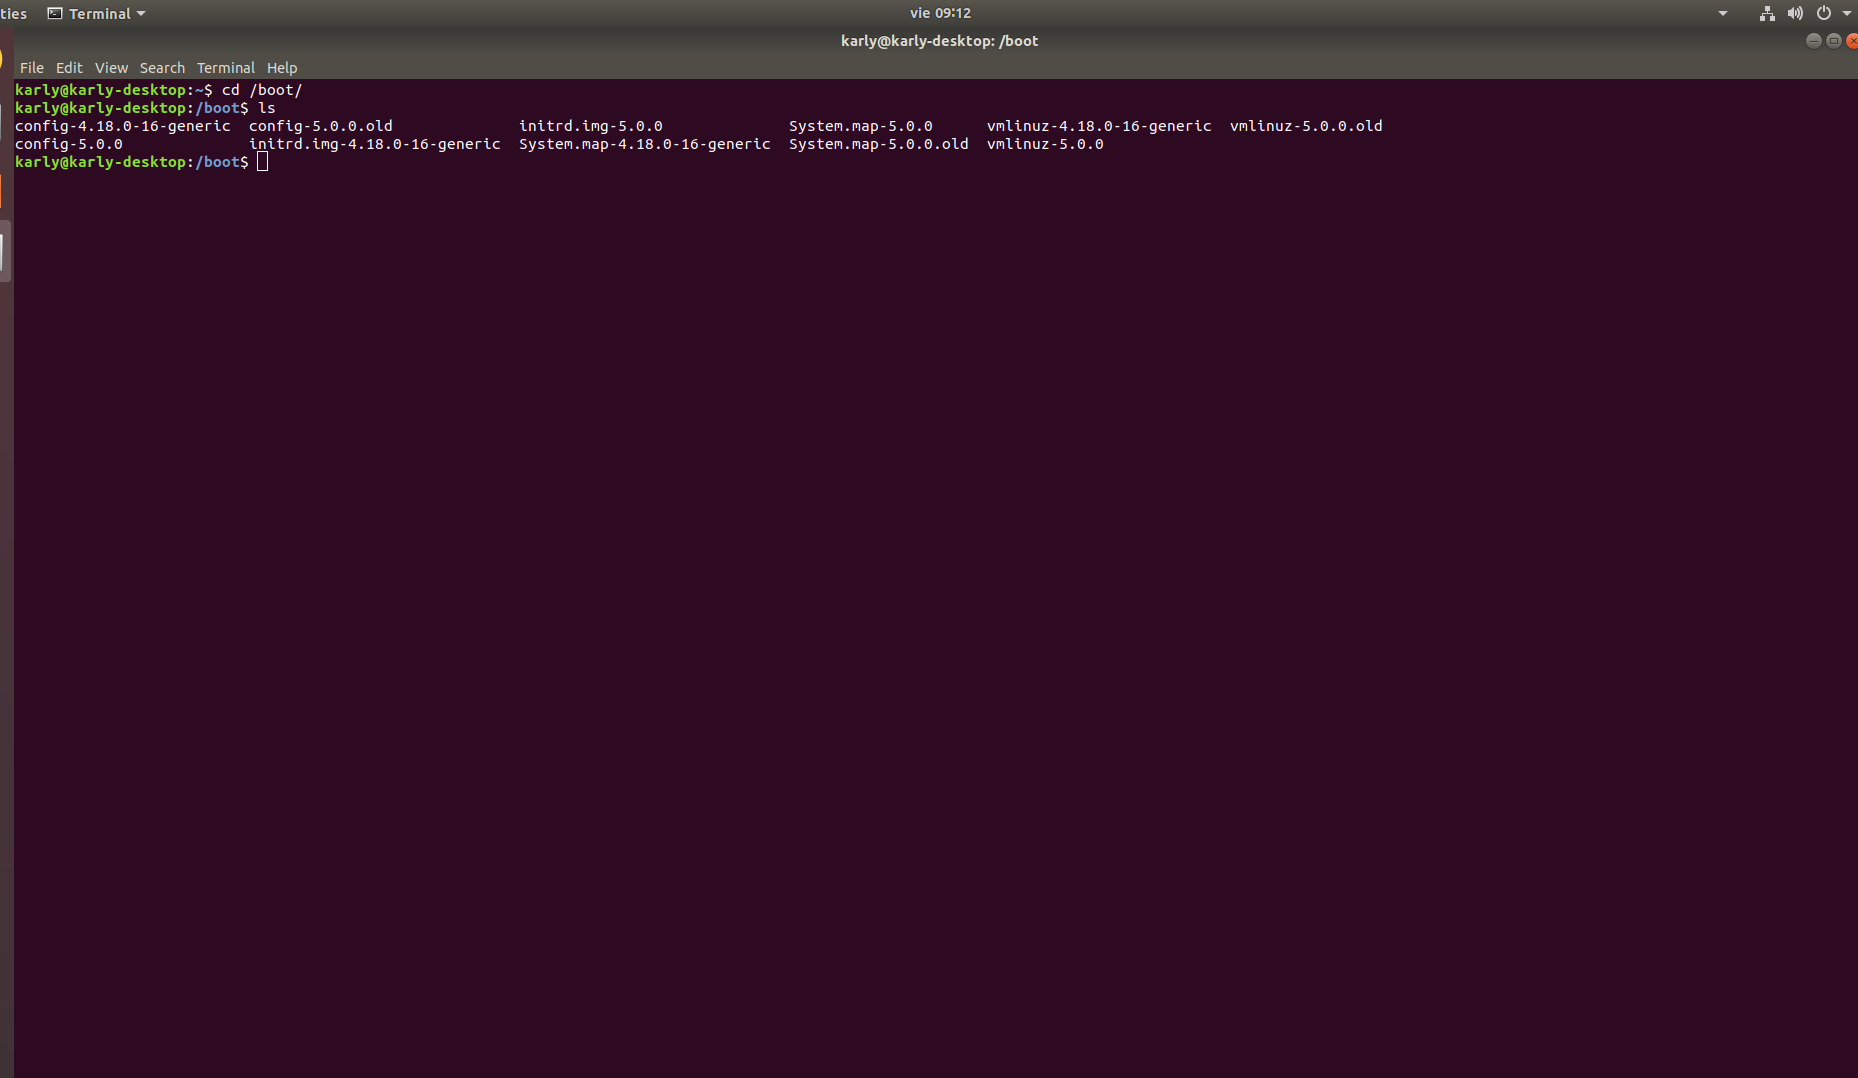
\includegraphics[scale=0.18]{config.png}
        Archivos de configuración.
    \end{center}
    \item Se tiene que instalar todas las herramientass necesarias para poder compilar para ello simplemente lo descargamos con el siguiente comando: \textbf{sudo apt-get install build-essential libncurses-dev bison flex libssl-dev libelf-dev}
    \item Hay que hacer una pequeña modificación al sistema, en mi caso como utilizo ubuntu sino se hace presentan algunos erroes a la hora de compilar, hay que marcar las siguientes opciones:
    \begin{center}
        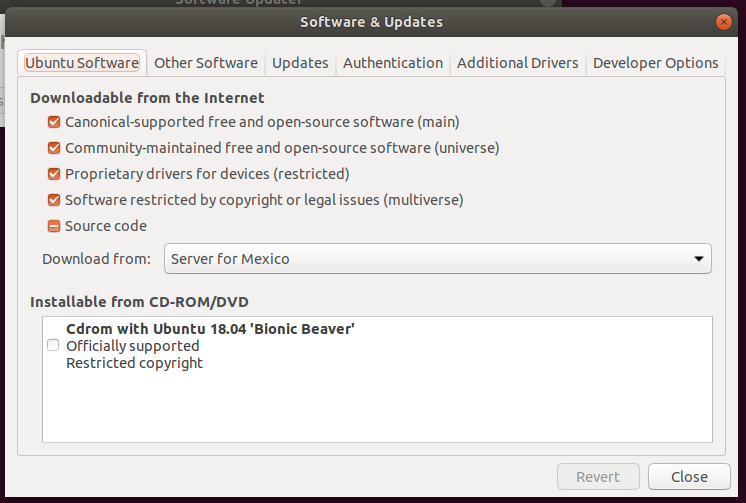
\includegraphics[scale=0.40]{modif.png}
    \end{center}
    \item Se configura el sistema
    \begin{itemize}
        \item \$ make menuconfig - Menús de colores, radiolistas y diálogos basados en texto. Esta opción también es útil en el servidor remoto si desea compilar el kernel de forma remota.
        \item \$ make xconfig - Herramienta de configuración basada en X windows (Qt), funciona mejor en el escritorio KDE
        \item \$ make gconfig - La herramienta de configuración basada en X windows (Gtk), funciona mejor bajo Gnome Dekstop.
        
    \end{itemize}
    En otro caso también en otro caso se puede utilizar el comando 
    make menuconfig que abre una ventana para que puedas hacer las modificaciones deseadas-
    \item para compilar el kernel simplemente se utiliza el comando \textbf{make}
    \begin{center}
        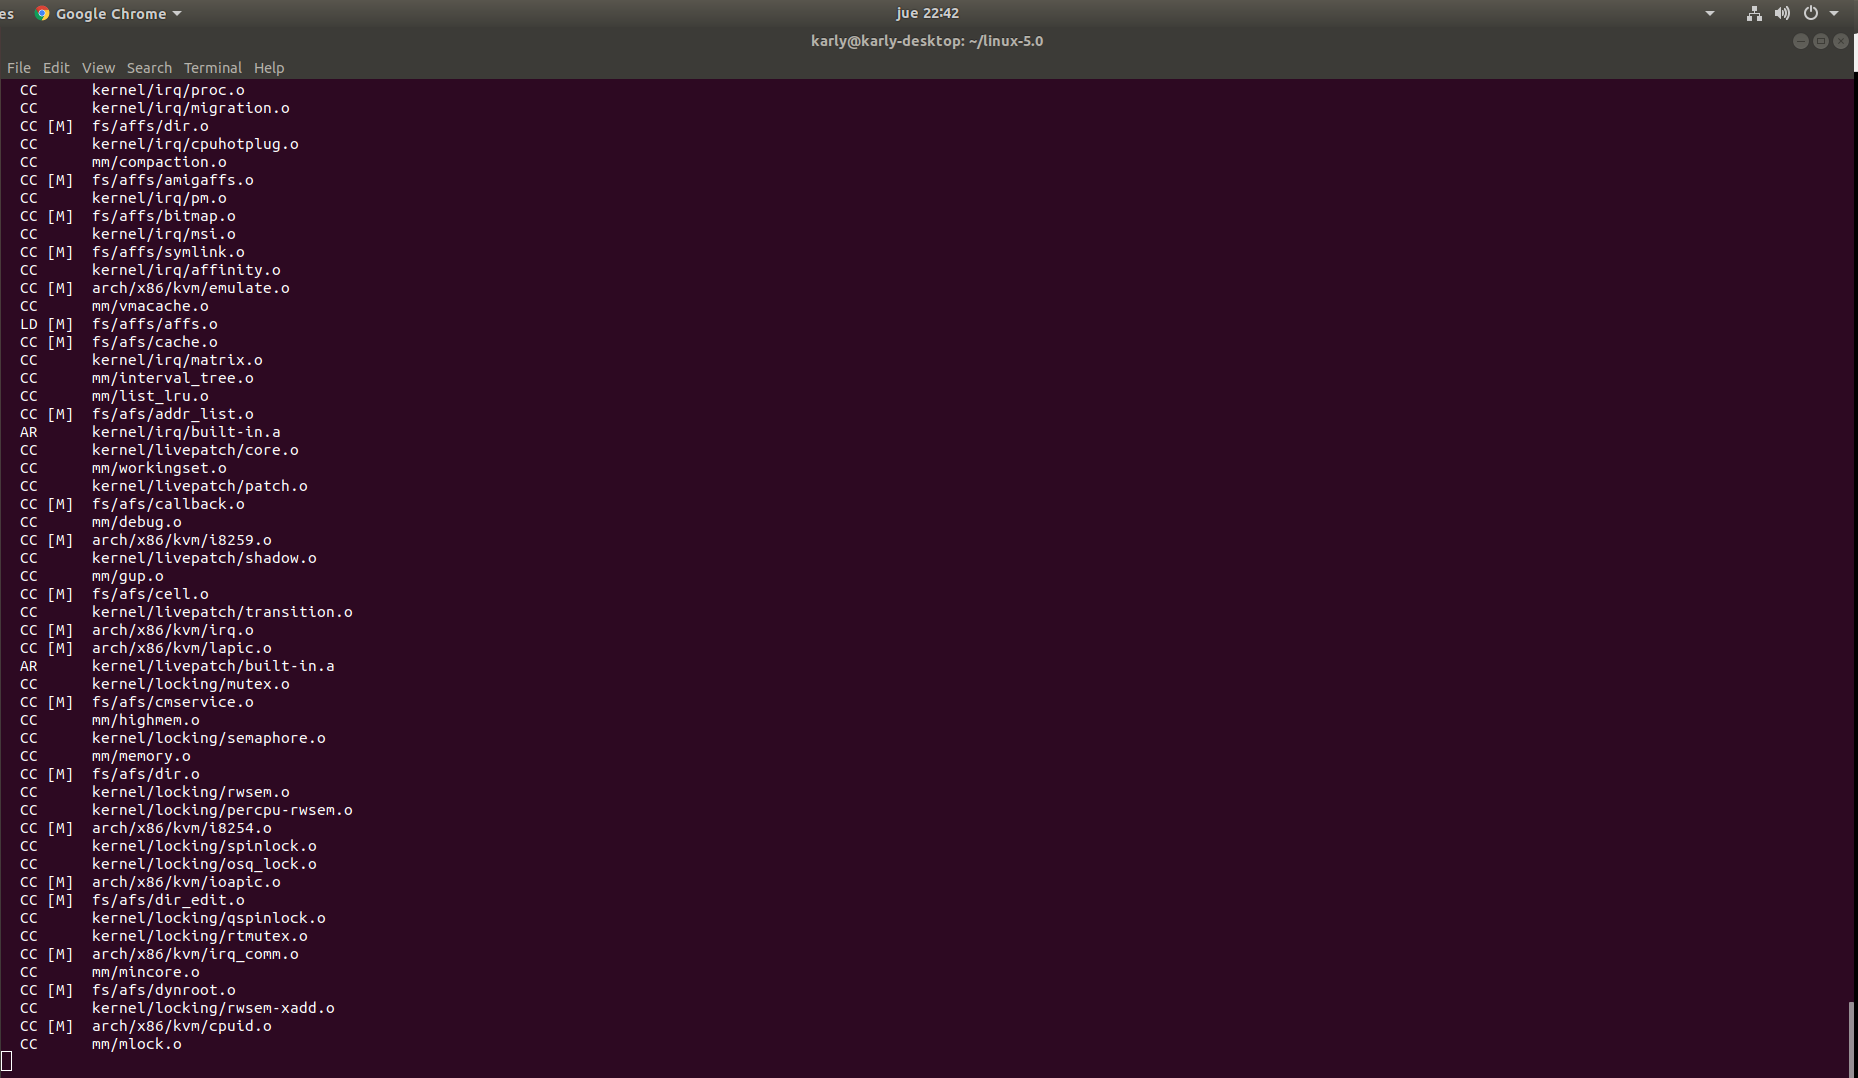
\includegraphics[scale=0.15]{compilacion.png}
        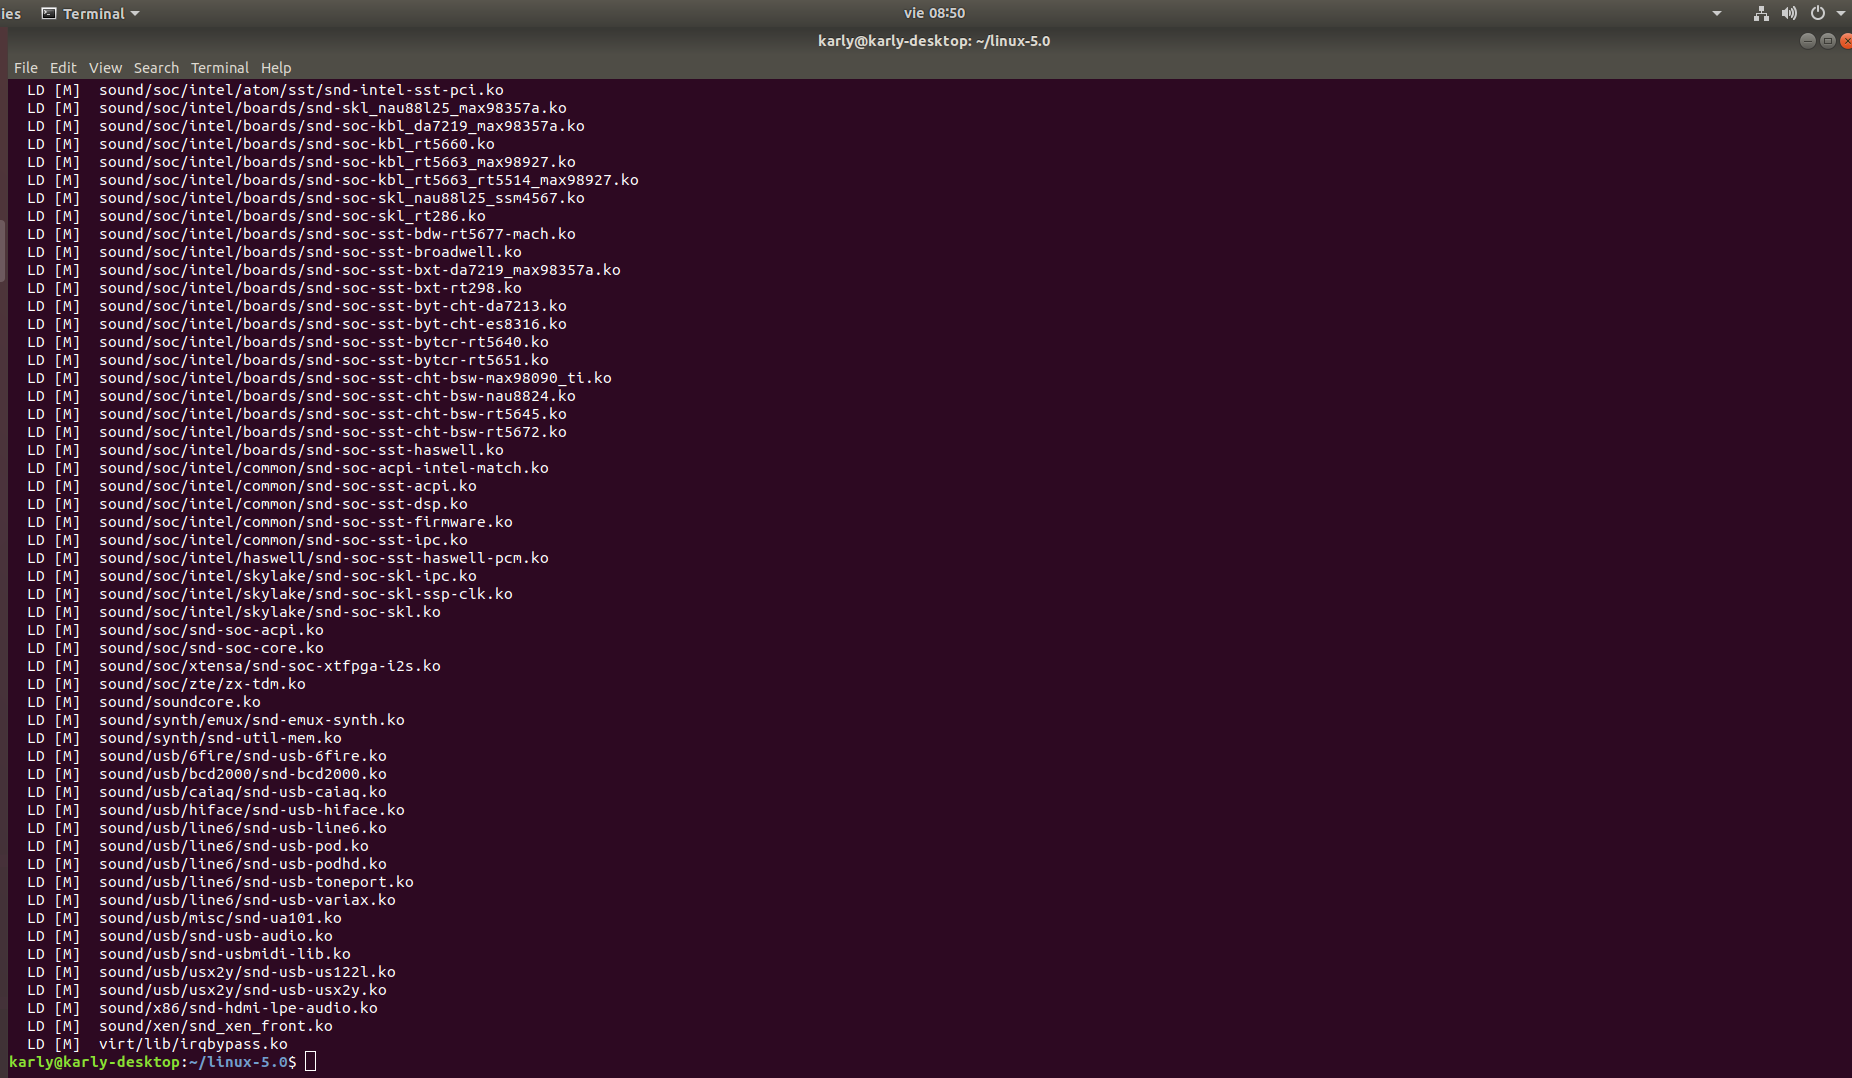
\includegraphics[scale=0.18]{compilacion0.png}
    \end{center}
    \item para instalar los módulos una vez que termine de compilar el kernel se utiliza el comando \textbf{sudo make modules\_install}
    \begin{center}
        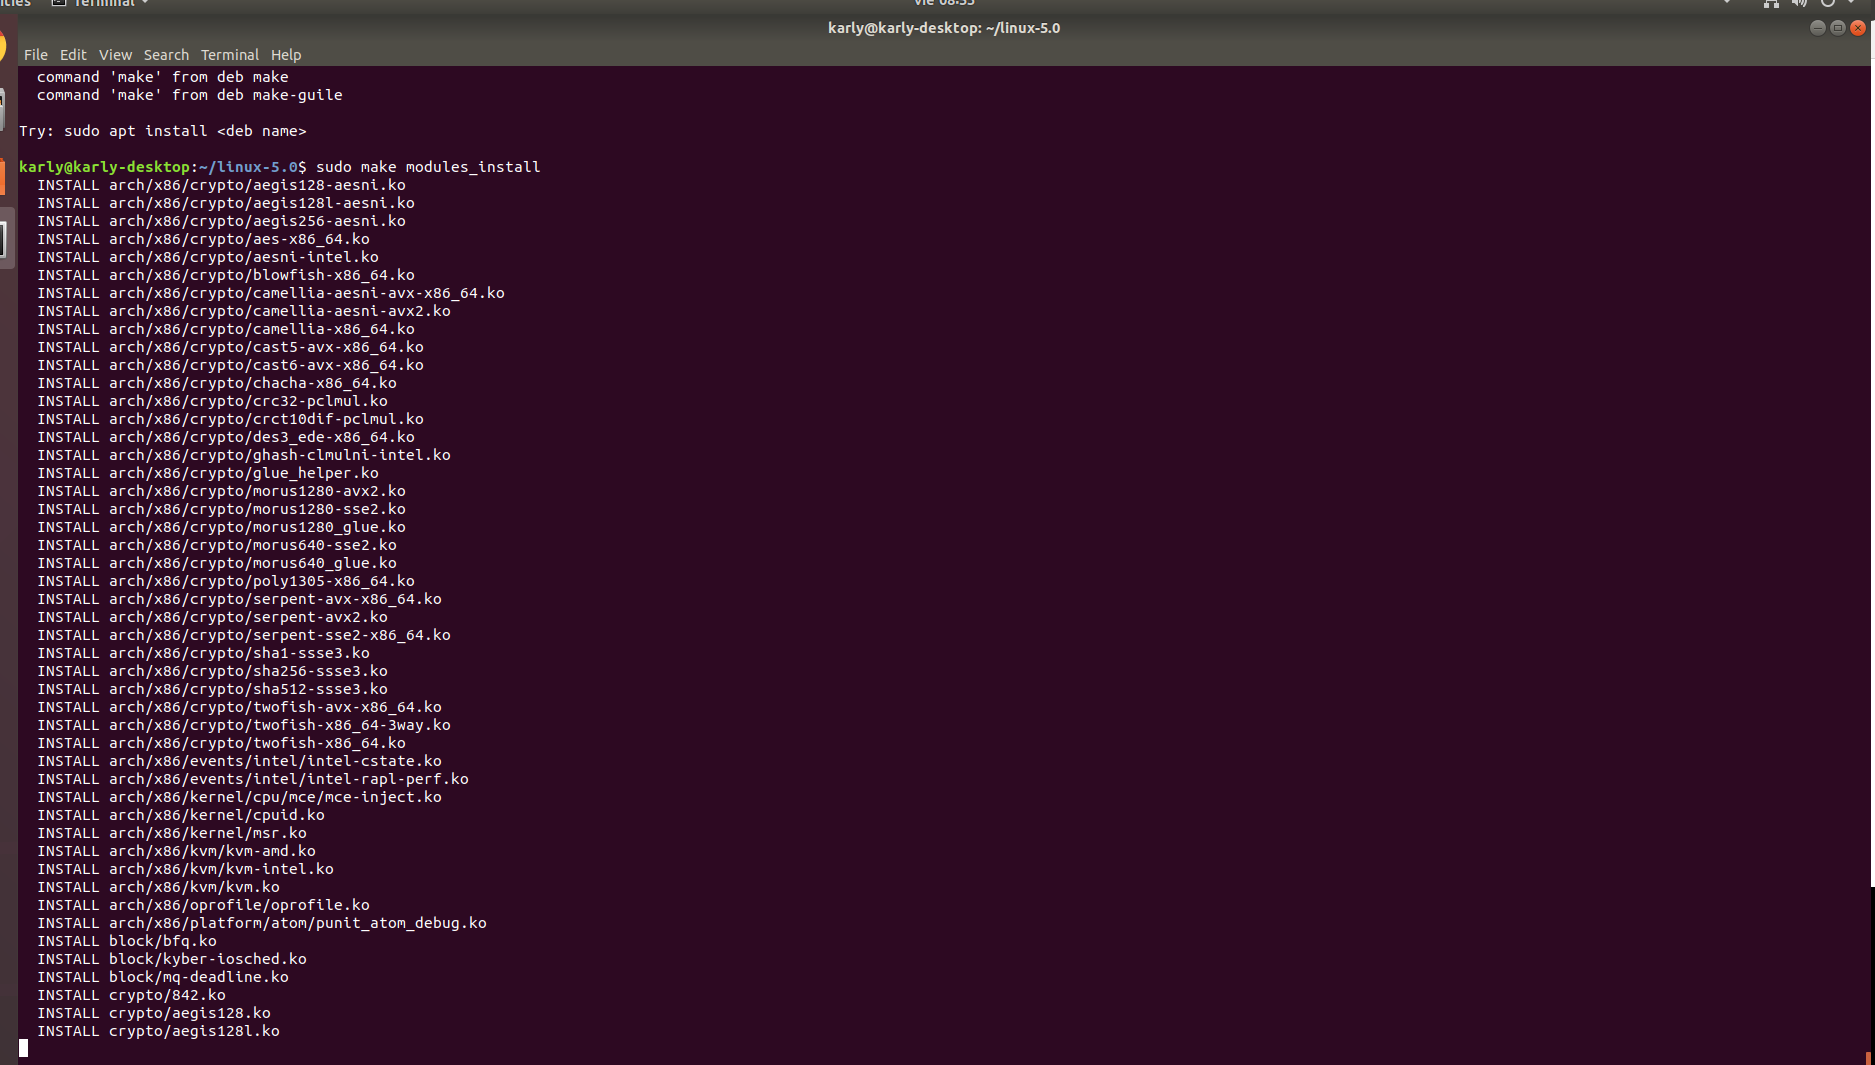
\includegraphics[scale=0.18]{Instalacionmodulos.png}
        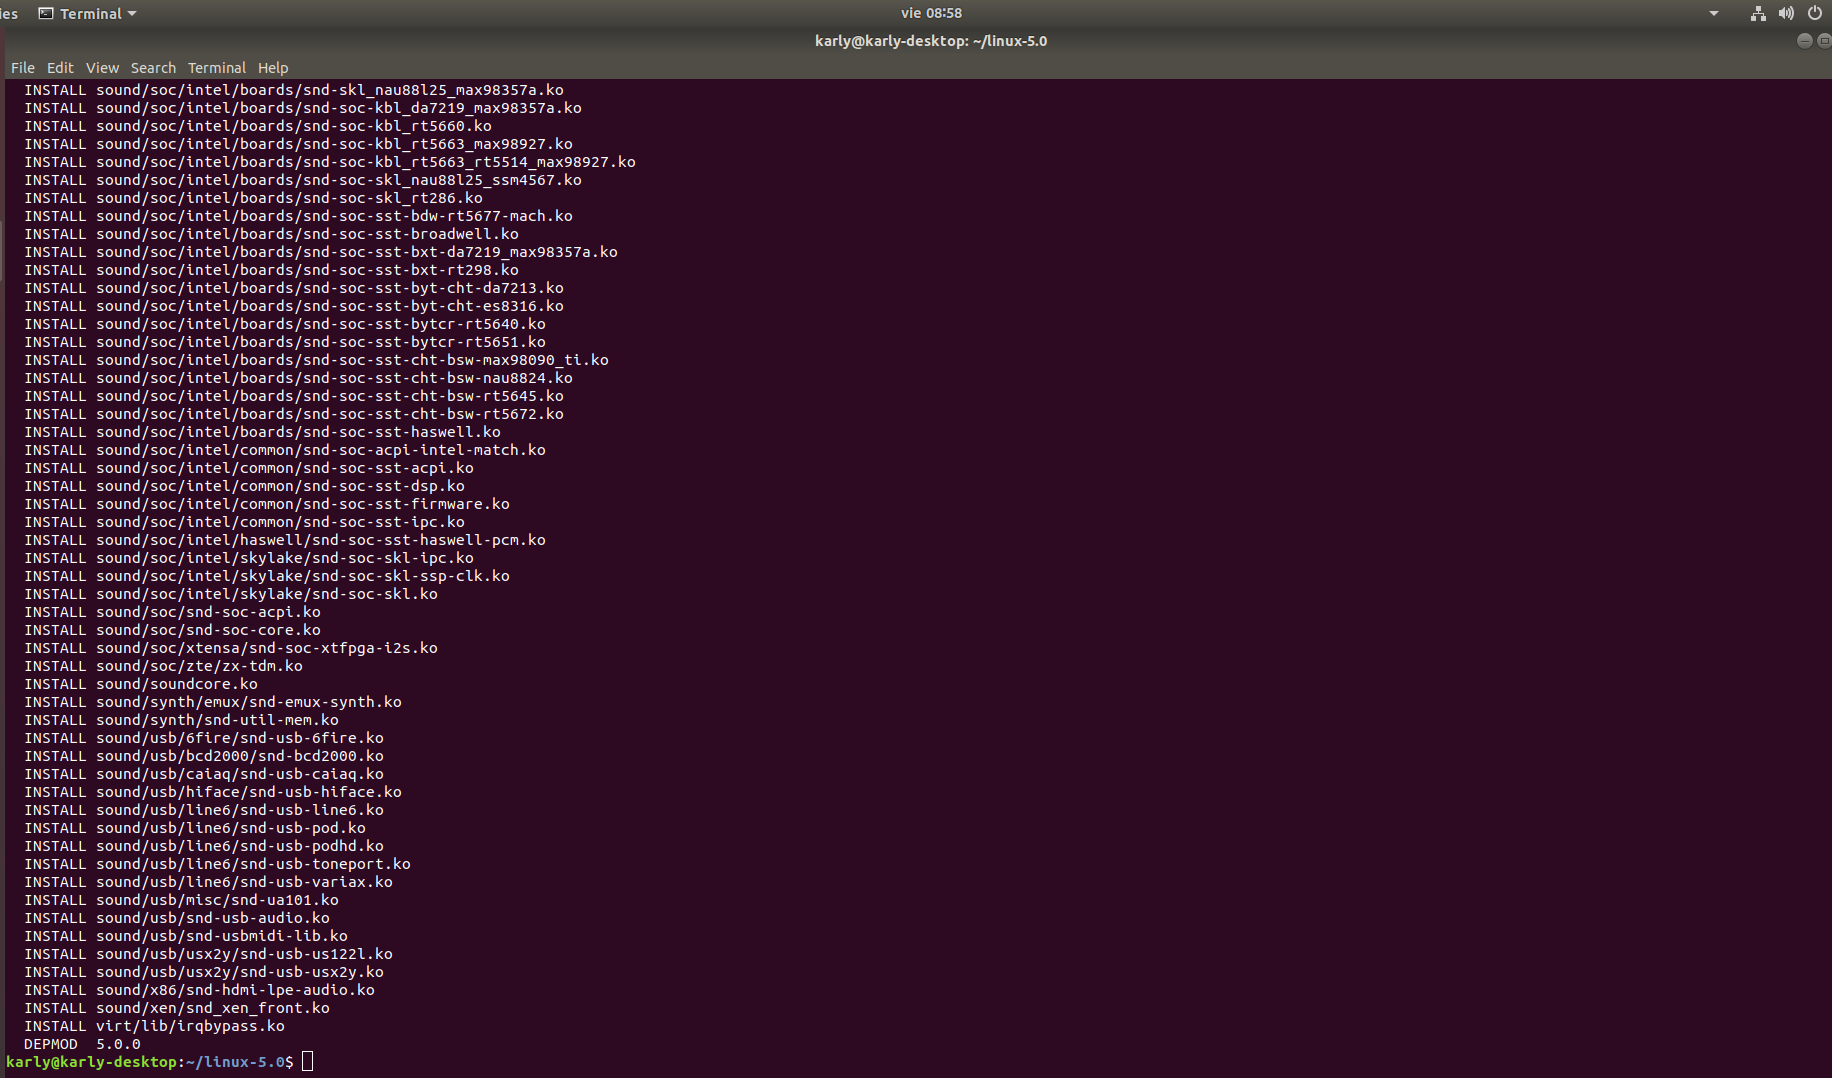
\includegraphics[scale=0.18]{Instalacionmodulos2.png}
    \end{center}
    \item Finalmente para instalar el kernel se utiliza el comando
    \textbf{sudo make install}.
    \begin{center}
        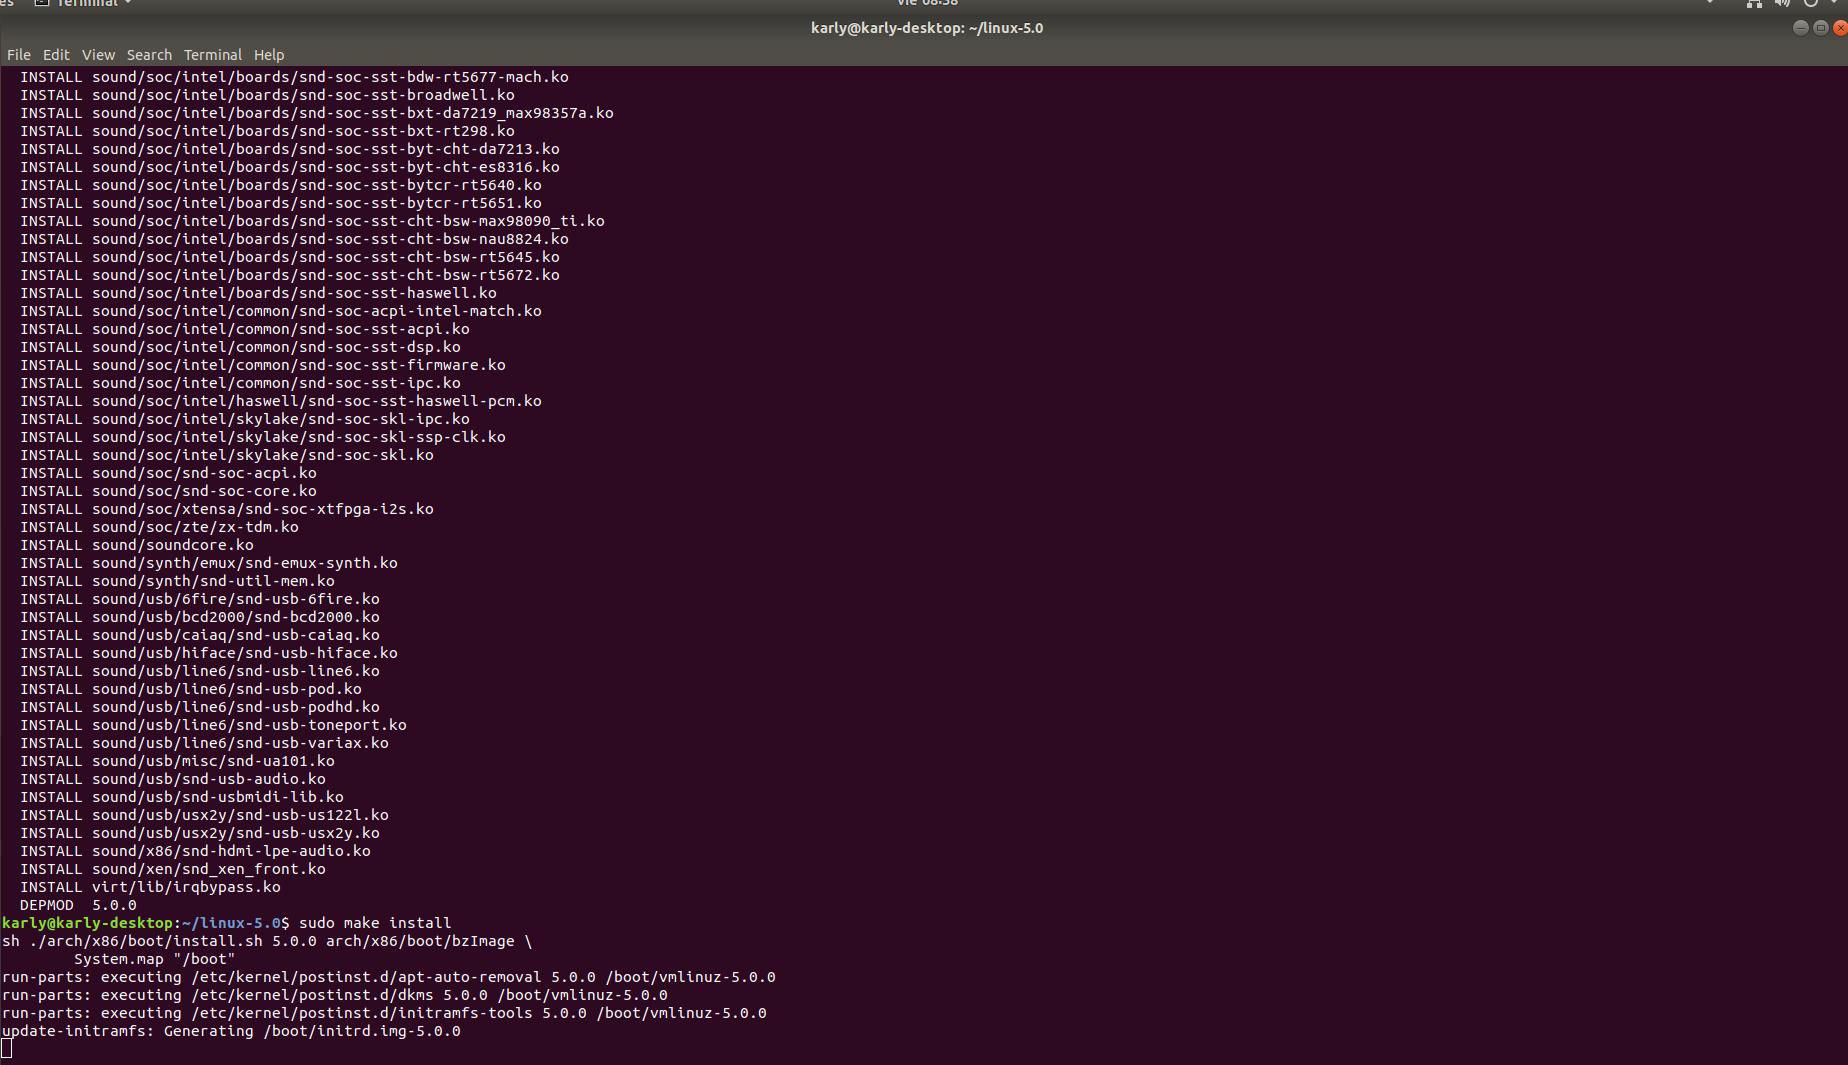
\includegraphics[scale=0.18]{Installkernel.png}
        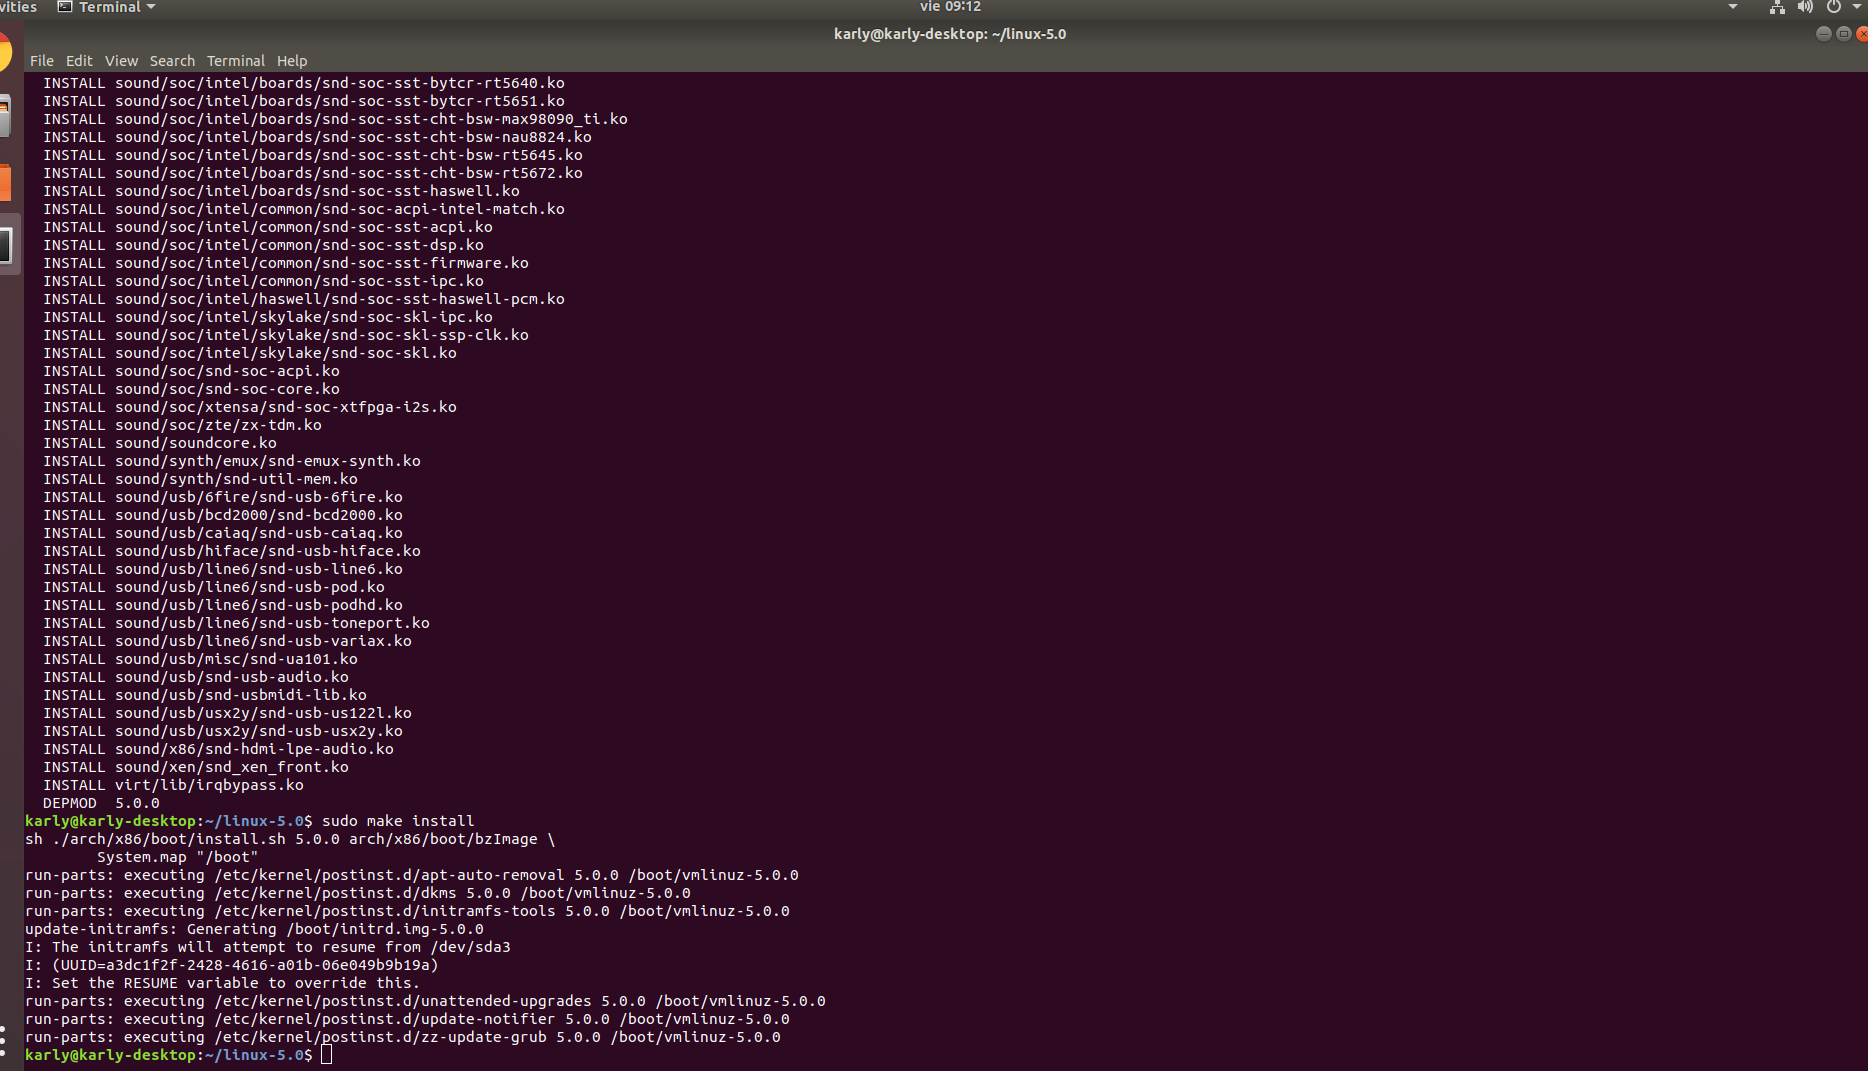
\includegraphics[scale=0.18]{kernel.png}
    \end{center}
\end{enumerate}
\end{document}